\documentclass[11pt]{article}
\usepackage[T1]{fontenc}
\usepackage[utf8]{inputenc}
\usepackage{lmodern,microtype}
\usepackage[margin=1.05in]{geometry}
\usepackage{amsmath,amssymb,amsthm,mathtools}
\usepackage{enumitem,graphicx,booktabs,array}
\usepackage{tikz}
\usetikzlibrary{arrows.meta,positioning,calc}
\usepackage[numbers,sort&compress]{natbib}
\usepackage{xurl}
\usepackage[colorlinks=true,linkcolor=blue!45!black,citecolor=blue!45!black,urlcolor=blue!45!black]{hyperref}
\usepackage[capitalise,noabbrev]{cleveref}
\usepackage{bookmark}
\pdfinfoomitdate=1
\pdftrailerid{}
\pdfsuppressptexinfo=15
\input{glyphtounicode}
\input{glyphtounicode-cmex}
\pdfgentounicode=1
\hypersetup{pdftitle={Regular trajectories, pruning and quantum parity},pdfauthor={OpenAI},pdfsubject={Constant-depth quantum circuits and bounded-error parity},bookmarksdepth=2}
\newtheorem{theorem}{Theorem}[section]
\newtheorem{lemma}[theorem]{Lemma}
\newtheorem{proposition}[theorem]{Proposition}
\newtheorem{corollary}[theorem]{Corollary}
\theoremstyle{definition}
\newtheorem{definition}[theorem]{Definition}
\theoremstyle{remark}
\newtheorem{remark}[theorem]{Remark}
\numberwithin{equation}{section}
\newcommand{\QAC}{\mathsf{QAC}^{0}}
\newcommand{\Parity}{\mathrm{PARITY}}
\newcommand{\C}{\mathbb C}
\newcommand{\one}{\mathbf 1}
\DeclarePairedDelimiter{\norm}{\lVert}{\rVert}
\DeclarePairedDelimiter{\abs}{\lvert}{\rvert}
\newcommand{\ip}[2]{\langle #1,#2\rangle}
\DeclareMathOperator{\Tr}{Tr}
\DeclareMathOperator{\supp}{supp}
\setlist[enumerate]{itemsep=.3em,topsep=.5em}
\setlist[itemize]{itemsep=.2em,topsep=.4em}
\setlength{\emergencystretch}{1.5em}
\title{Regular trajectories, pruning and quantum parity}
\author{OpenAI}
\date{September 24, 2026}
\begin{document}
\maketitle
\begin{abstract}
We prove that constant-depth quantum circuits with arbitrary one-qubit
gates and unbounded-arity Toffoli gates cannot compute parity with
any fixed positive worst-case advantage using polynomially many total
qubits. Ancillary qubits are initialized to $|0\rangle$, one output qubit
is measured, and all other final registers may be discarded without
restriction. This resolves Moore's parity conjecture in the
measured-output model.
\end{abstract}
\setcounter{tocdepth}{1}
\tableofcontents
\section{Introduction}
\label{sec:introduction}

The class $\QAC$ consists of constant-depth quantum circuits with
arbitrary one-qubit gates and generalized Toffoli gates of unbounded
arity, using polynomially many total qubits. Ancillary qubits are initialized
to zero.
The supports of gates in a layer are pairwise disjoint. This last
condition makes the availability of fanout a substantive question:
one cannot simultaneously use a qubit as the control of arbitrarily
many two-qubit gates. Moore asked whether the coherent fanout
operation can be implemented in this model, and conjectured a
negative answer. Its unitary parity counterpart is equivalent
by Hadamard conjugation
\citep{Moore1999,GreenHomerMoorePollett2002}.

We prove Moore's parity conjecture in the measured-output model and
therefore also exclude coherent fanout. The lower bound
holds for bounded-error computation with a single measured output,
even when the computation changes the input and leaves arbitrary
garbage in the other registers.

\subsection{The circuit model and the result}

For $x\in\{0,1\}^{n}$, let
\[
  \Parity_n(x)=x_1\mathbin{\oplus}\cdots\mathbin{\oplus}x_n.
\]
An allowed circuit acts on $\lvert x\rangle\lvert0\rangle^{\otimes a}$.
Its gates are arbitrary one-qubit unitaries and generalized Toffoli
gates
\[
 \lvert z_1,\ldots,z_t,b\rangle
 \longmapsto
 \lvert z_1,\ldots,z_t,b\mathbin{\oplus}(z_1\cdots z_t)\rangle,
 \qquad t\ge1,
\]
on distinct control and target qubits. Each gate has unit cost,
regardless of its arity. A depth-$d$ circuit is a product of $d$
layers of gates with pairwise disjoint supports. There is no
geometric restriction. At the end, one designated qubit is measured
in the computational basis. The other registers may be discarded.
Intermediate measurements, postselection, and additional fanout
gates are not allowed. All gates and their complex entries may
depend arbitrarily on $n$, but not on $x$.

\begin{theorem}
\label{thm:parity}
Fix positive integers $d,k,C$ and a real $0<\varepsilon\le1/2$.
There is an integer $n_0=n_0(d,k,C,\varepsilon)$ such that,
for every $n\ge n_0$, every allowed circuit of depth at most $d$
on at most $C(n+1)^k$ total qubits has an input $x\in\{0,1\}^{n}$ on which its answer equals
$\Parity_n(x)$ with probability strictly less than $1/2+\varepsilon$.
\end{theorem}

Here total qubits means the $n$ inputs together with all ancillary
qubits. Disjoint nonempty gate supports imply that a depth-$d$ circuit
on $N$ qubits contains at most $dN$ gates. Thus the theorem covers the
usual fixed-depth model with polynomially many gates and polynomially
many ancillas: the ancillary bound gives a polynomial bound on $N$,
and a polynomial bound on $N$ already bounds the number of gates.

In particular, no nonuniform constant-depth family with polynomial
resources computes parity with any fixed positive worst-case advantage.
The theorem is eventual for each fixed depth, polynomial bound, and advantage;
it permits arbitrary finite exceptions at small input lengths.

To make the connection with fanout explicit, let
\[
 F_n\lvert y_1,\ldots,y_n,b\rangle
 =\lvert y_1\mathbin{\oplus}b,\ldots,
          y_n\mathbin{\oplus}b,b\rangle.
\]
For the Hadamard gate $H$, conjugating a controlled-NOT by
$H\otimes H$ interchanges its control and target; this follows
directly from its action on the two-qubit basis. Writing $F_n$
as the product of its commuting controlled-NOT operations gives
\[
 H^{\otimes(n+1)}F_nH^{\otimes(n+1)}
 \lvert y,b\rangle
 =\lvert y,b\mathbin{\oplus}\Parity_n(y)\rangle.
\]
Thus a constant-depth polynomial-resource implementation of
$F_n$, together with two layers of one-qubit gates and a zero
target, would contradict Theorem~\ref{thm:parity}. This also
excludes Moore's original formulation, in which the ancillary
qubits must be restored to zero \citep{Moore1999}.

Theorem~\ref{thm:parity} also has state-preparation consequences
corresponding to those of Gretta, Gupta, and Joshi
\citep[Corollary~4.10 and Theorem~4.14]{GGJ2026Fourier}.
Let $\rho$ be the retained $n$-qubit state of an allowed unitary
preparation from all-zero inputs, with arbitrary final ancillas discarded.
Its felinity is $2\sum_y p_y p_{\bar y}$, where
$p_y=\langle y|\rho|y\rangle$ and $\bar y$ is the bitwise complement of $y$.
At each fixed depth and fixed polynomial total-qubit bound, for every fixed
$A>0$, eventually every such preparation has felinity less than $n^{-A}$.
For every fixed $0<\delta<1$, eventually every such preparation and every
integer $k$ with $n^\delta\le k\le n/2$ also satisfy
\[
 \tfrac12\bigl\|\rho-|D_k^n\rangle\langle D_k^n|\bigr\|_1
 >\frac1{80k},
 \qquad
 |D_k^n\rangle=\binom nk^{-1/2}\sum_{|y|=k}|y\rangle.
\]
Here trace distance is one half of the trace norm. The companion states
the same bounds
\citep[Corollary~8 (State-preparation obstructions), Section~7.1]{OpenAILocalization2026}.
The argument after the parity proof in Section~\ref{sec:parity}
justifies the pointwise reductions, including exact promotion with
arbitrary final garbage and polynomial total-qubit overhead.

\subsection{Previous work}

The classical class $\mathsf{AC}^{0}$ allows unbounded-fan-in AND and
OR gates, NOT gates, and unrestricted reuse of wires. Parity was among
the first explicit functions shown to require superpolynomial size
at constant depth, by Furst, Saxe, and Sipser and independently Ajtai
\citep{FurstSaxeSipser1984,Ajtai1983}; H\aa stad obtained almost optimal
exponential bounds through the switching lemma \citep{Hastad1986}.
The quantum question combines the additional expressive power of
one-qubit unitaries with the disjoint-support restriction on each layer.
Moore's formulation and the counting classes studied by Green, Homer,
Moore, and Pollett made the role of coherent fanout explicit
\citep{Moore1999,GreenHomerMoorePollett2002}. Constant-depth
constructions with fanout further demonstrated the computational
importance of that operation \citep{HoyerSpalek2005}.

Early quantum lower bounds exposed the importance of the ancillary
register. Fang, Fenner, Green, Homer, and Zhang proved a depth bound of
order $\log(n/(a+1))$ for exact parity computation with $a$ ancillas
that must be restored to zero
\citep[Corollary~4.6]{FangFennerGreenHomerZhang2006}.
Pad\'e, Fenner, Grier, and Thierauf ruled out exact clean simulation
at entangling depth two \citep{PadeFennerGrierThierauf2020}; Fenner,
Grier, Pad\'e, and Thierauf subsequently removed the final-state
cleanliness requirement for exact single-output parity at that depth
\citep[Theorem~6.1]{FennerGrierPadeThierauf2025}.
Here and in the depth-specific comparisons below, \emph{entangling
depth} counts only layers of multiqubit gates; arbitrary one-qubit
layers may occur between them. This convention differs from our total
layer count by at most a constant factor for fixed depth.

Rosenthal obtained lower bounds for approximate parity and fanout
unitaries and related cat-like states, together with constant-depth
approximation constructions using superpolynomial resources
\citep{Rosenthal2021}. Approximation of a parity unitary is a stronger
task than computing one measured classical bit: the latter may destroy
the input and leave arbitrary garbage. Nadimpalli, Parham, Vasconcelos,
and Yuen developed Pauli-spectrum methods with depth-dependent
restrictions on the ancillary count
\citep{NadimpalliParhamVasconcelosYuen2024}. Anshu, Dong, Ou, and Yao
obtained lower bounds allowing barely superlinear ancillary counts
\citep{AnshuDongOuYao2025}; Dong, Ou, and Yao developed further
low-degree estimates and applications to quantum channels
\citep{DongOuYao2025}. These resource restrictions do not cover an
arbitrary fixed polynomial ancillary bound.

Joshi, Tal, Vasconcelos, and Wright ruled out exact parity at
entangling depth three for sufficiently large input lengths, with no
bound on the number of gates or ancillas. They also proved approximate
parity lower bounds at entangling depth two for one measured output,
without requiring input preservation
\citep{JoshiTalVasconcelosWright2025}. Kintali's September 2026
preprint reports exponentially small average parity correlation at
entangling depth at most three, independently of the number of gates
and ancillas, and an exponential gate lower bound for exact parity at
entangling depth at most four
\citep[Theorems~1--2]{Kintali2026ShallowParity}.\footnote{Joshi et al.
acknowledge ChatGPT's contribution to a lemma's proof idea and other
interactions; Kintali discloses assistance from Claude, ChatGPT, and
two open-weight models. Neither source specifies model versions.}
These depth-specific statements do not cover every fixed depth.
Gretta, Gupta, and Joshi characterize the general parity question
through Fourier concentration \citep{GGJ2026Fourier}, while Xu and Li
extend related fanout reductions to symmetric functions
\citep{XuLi2026Fanout}. Our theorem permits every fixed depth and
every polynomial total-qubit bound simultaneously. All structural
statements needed for its proof are established below.

The companion article \emph{Product-projection localization and the
QAC0 parity lower bound} proves a uniform operator-norm localization
theorem and an independent parity lower bound
\citep[Sections~2 and~6]{OpenAILocalization2026}. The present article instead
proves state-dependent propagation, projection insertion, and pruning
for regular trajectories. Both arguments use product-projection counts
and elementary Chebyshev filters; neither structural theorem is used
to prove the other.

\subsection{The proof and its main tools}

A generalized Toffoli gate is a reflection $I-2P$, where $P$ is a
product of one-qubit rank-one projections. This representation suggests
counting how many local factors of a product test fail. A single such
gate can couple arbitrarily many qubits, so its conjugation need not
preserve small operator support. Moreover, product-projection filters
can have large norms away from the count range where they approximate
well. Controlling the state on which each approximation is used is
therefore essential.
Informally, a trajectory sequence is \emph{regular} when, for every
sufficiently small collection of reflections in a layer, the combined count
of failures of their local factors has a rapidly decaying tail on the state
entering that layer. The precise definition is asymptotic and allows
arbitrary gates and states at each circuit size.

Polynomial locality and concentration have been related in work of
Kuwahara, Arad, Amico, and Vedral and of Anshu and Metger
\citep{KuwaharaAradAmicoVedral2017,AnshuMetger2023}. In the circuit
setting, Pauli concentration and low-degree approximation are central
to the works just discussed. An operator has degree at most $\ell$ when it is a sum of operators
supported on at most $\ell$ sites each. We retain the elementary link
between this degree and the number of product-basis coordinates an
operator can change. The additional steps here are two-sided tail transport and
stability under a product projection, which permit a trajectory to be
made regular by a state-dependent pruning rule.

The first tool, Proposition~\ref{prop:propagation}, transports
operators of low degree along a regular
trajectory, with an arbitrarily small fixed loss in the degree
exponent. Its conclusion is an approximation on the trajectory
vector. The second tool, Proposition~\ref{prop:projection-insertion},
shows that regularity survives insertion
of an arbitrary product projection followed by reverse evolution.
The key step is Lemma~\ref{lem:tail-transport}, which compares two
regular trajectories. One polynomial detects a tail at the starting end;
another approximates the product projection at the finishing end.
They are applied on different sides of an inner product, so their
large global norms are paid for by the appropriate tail estimates.

Projection stability then makes regularity available without an
initial assumption on the circuit. Starting from a product state,
we retain a reflection when its projection has probability at least
$m^{-6}$ on the current state, where $m$ is the number of qubits.
The retained layer is regular, and the deleted gates change the
state by at most $2m^{-2}$ per layer. Iterating this rule yields a
regular trajectory close to the original evolution
(Proposition~\ref{prop:pruning}). The stability
and propagation statements concern arbitrary product tests and
regular trajectories, rather than parity alone.

Finally, we copy each basis input into a reference register that the
subsequent computation leaves untouched.
On the uniform coherent input, worst-case parity success becomes
a signed acceptance expectation bounded away from zero. The
pruned circuit has almost the same expectation. Write $W$ for that circuit,
$\psi_0$ for the initial product state, and $P_B$ for the accepting output
projection. The copying gates survive pruning, so conjugating the reference
sign back through $W$ sends $\psi_0$
to a vector with exactly $n$ excitations relative to the initial product state
$\psi_0$. The signed expectation pairs this vector with $W^\dagger P_BW\psi_0$,
whose tail for that same count is bounded by
Corollary~\ref{cor:product-tail}. Because the total number $m$ of qubits is polynomially
bounded in $n$, a sufficiently small fixed $h>0$ can be chosen
with $m^h=o(n)$, separating these two scales and giving the contradiction.

Sections~\ref{sec:framework} and~\ref{sec:filters} introduce the
formalism and the polynomial filters. Section~\ref{sec:propagation}
proves low-degree propagation, and Section~\ref{sec:transport}
establishes tail transport. Projection stability and pruning are
proved in Section~\ref{sec:pruning}; Section~\ref{sec:parity}
completes the parity argument.

\section{Product tests and regular trajectories}
\label{sec:framework}

We work on the Hilbert space $(\C^2)^{\otimes m}$.  Vector norms are
Euclidean norms, and operator norms are the induced norms.  Unless explicitly
stated otherwise, every starting vector has norm at most one.  Products of
orthogonal projections used in the analysis are applied without renormalizing
the resulting vectors.
All projection insertions below are analytic devices; the permitted
circuit operations remain unitary until the final output measurement.

\subsection{The gate model and product tests}

The physical circuit has $n$ input qubits, $a$ ancillary qubits initialized to
$\lvert0\rangle^{\otimes a}$, and a designated output qubit measured in the
computational basis.  Its gates are arbitrary one-qubit unitaries and the
generalized Toffoli gates of Section~\ref{sec:introduction}.  Gates in each layer have pairwise
disjoint supports, and each gate counts once regardless of its arity.
The gates may depend arbitrarily on the input length,
including through their complex entries, but are independent of the input
string.  No input or ancillary register is required to be restored, and the
output qubit may be an original input qubit.  All other qubits may be discarded
after the output is measured.  There are no intermediate measurements,
postselection operations, geometric restrictions, or extra fanout gates.

For the analysis, we allow a reflection
\[
 R_g=I-2P_g,
 \qquad
 P_g=\bigotimes_{j\in J_g}\lvert v_{g,j}\rangle\langle v_{g,j}\rvert
       \otimes I_{J_g^c},
\]
where $J_g$ is a nonempty set of sites and each $v_{g,j}$ is a unit vector.
The tensor factors are understood to occupy their indicated sites.  Each
$P_g$ is an orthogonal projection, so $R_g=R_g^\dagger=R_g^{-1}$.
A generalized Toffoli with $c\ge1$ distinct controls $z_1,\ldots,z_c$ and
a distinct target $b$ has this form with
\[
 P_g=\left(\bigotimes_{i=1}^{c}\lvert1\rangle\langle1\rvert_{z_i}\right)
       \otimes\lvert-\rangle\langle-\rvert_b,
 \qquad
 \lvert-\rangle=\frac{\lvert0\rangle-\lvert1\rangle}{\sqrt2},
\]
and identities elsewhere.  Indeed, it acts trivially unless all controls are
one, and on that control subspace its target action is
$I-2\lvert-\rangle\langle-\rvert=X$.
This product-reflection viewpoint also appears in
\citet{Rosenthal2021}.

An \emph{analytic layer} will be either a product of such reflections on
pairwise disjoint supports, or a tensor product of one-qubit unitaries.
Splitting a physical layer into its two gate types preserves its operation,
because its gates have disjoint supports.  Thus a physical circuit of depth
$d$ gives at most $2d$ analytic layers.  We use $t$ for their number and $m$
for the total number of qubits, including any reference qubits subsequently
introduced.  Empty layers are permitted.  Every reflection layer has at most
$m$ gates, since their supports are nonempty and disjoint.

\begin{definition}[Product test]
\label{def:test}
A test $A$ consists of a subset $J_A\subseteq\{1,\ldots,m\}$ and a specified
unit vector $v_{A,j}$ at each $j\in J_A$.  Its excitation count and zero
projection are
\[
 H_A=\sum_{j\in J_A}
       \bigl(I-\lvert v_{A,j}\rangle\langle v_{A,j}\rvert\bigr)_j,
 \qquad
 P_A=\one_{H_A=0}
    =\bigotimes_{j\in J_A}\lvert v_{A,j}\rangle\langle v_{A,j}\rvert
       \otimes I_{J_A^c}.
\]
Here a subscript $j$ extends a one-site operator by identity at all other
sites, and $\one_{H_A\in E}$ denotes the spectral projection of $H_A$ onto
the set $E\subseteq\mathbb R$.  The empty test has $H_A=0$ and $P_A=I$.
\end{definition}

The summands of $H_A$ are commuting orthogonal projections.  Choosing the
basis $(v_{A,j},v_{A,j}^{\perp})$ at each tested site diagonalizes them
simultaneously.  Consequently its spectrum is contained in
$\{0,1,\ldots,|J_A|\}$, and $0\le H_A\le mI$.  We use spectral inequalities
such as $H_A\ge x$ also when $x$ is not an integer.

For a set $S$ of gates in one reflection layer, disjointness makes their
specified local factors a single test.  We write $H_S$ for its count and
$P_S=\prod_{g\in S}P_g$ for its zero projection.  If $F$ is the whole
reflection layer, then
\[
 [F,H_S]=0.
\]
Indeed, a gate in $S$ commutes with each of its own local factors, while
other gates have disjoint supports.  Every spectral projection of $H_S$
therefore commutes with $F$ as well.  If $H_A$ retains only some sites of
this test, then $H_A$ and $H_S$ are diagonal in the same product basis,
$H_A\le H_S$, and
\[
 \one_{H_A\ge x}\le\one_{H_S\ge x}
 \quad\text{for every real }x.
\]

\subsection{Asymptotic sequences and uniformity}

All asymptotic statements concern an arbitrary sequence indexed by
$\nu\in\mathbb N$, with total qubit counts $m_\nu\to\infty$ and a bounded
number of analytic layers.  The states, tests, gates, and circuits can all
vary with $\nu$.  We suppress $\nu$ and write $m$ for $m_\nu$; thus
``eventually'' means at all sufficiently large sequence indices.  Every
exponent appearing in an estimate is a fixed real number independent of
$\nu$.  Padding with empty layers gives a common bound on length.  When a
fixed layer pattern is convenient, one may restrict to a subsequence with
fixed length and layer types: there are only finitely many such patterns.
An eventual assertion on every such subsequence yields the assertion on
the original sequence, since any infinite set of violations has an infinite
subsequence with one fixed pattern.

The following elementary observation will also supply uniformity over
tests chosen from the current state.

\begin{lemma}[Uniformity from arbitrary choices]
\label{lem:uniformization}
Fix a sequence of base data, and let $\mathcal D_\nu$ be the nonempty set of
permitted auxiliary choices at index $\nu$.  Suppose that for every sequence
$D_\nu\in\mathcal D_\nu$ and every fixed admissible parameter tuple
$\theta$, an assertion $\mathcal E(\nu,D_\nu,\theta)$ holds eventually.
Then, for every fixed $\theta$, there is an index $\nu_0$ such that
\[
 \mathcal E(\nu,D,\theta)
 \quad\text{holds for all }\nu\ge\nu_0
 \text{ and every }D\in\mathcal D_\nu.
\]
The same conclusion holds if the premise is proved on every subsequence
on which the base hypotheses remain valid.
\end{lemma}

\begin{proof}
Fix $\theta$.  If the conclusion fails, there are increasing indices
$\nu_i$ and choices $D_{\nu_i}\in\mathcal D_{\nu_i}$ violating the
assertion.  Choose arbitrary permitted values at the other indices.  The
resulting sequence of choices contradicts the premise.  In the subsequence
version, apply the premise directly to the violating subsequence.
\end{proof}

The lemma imposes no cardinality or finiteness requirement on
$\mathcal D_\nu$.  In particular, a permitted test may depend on the exact
state at its index.  The eventual threshold may depend on the fixed tuple
$\theta$; no threshold uniform over all real exponent tuples is asserted.

\begin{definition}[Regular trajectory]
\label{def:regular}
Write $V=U_t\cdots U_1$ for analytic layers and set
$\xi_j=U_j\cdots U_1\xi_0$, where $\norm{\xi_0}\le1$.
The sequence of these trajectories is \emph{regular} if the following
holds at every reflection layer $U_j$: for \emph{every fixed} triple
\[
 0\le b<h<1,\qquad 0<p<h,
\]
eventually, simultaneously for every set $S$ of at most $m^b$ gates of
that layer,
\begin{equation}
 \norm{\one_{H_S\ge m^h}\xi_{j-1}}
 \le \exp(-m^p).
 \label{eq:regularity}
\end{equation}
There is no regularity condition at one-qubit layers.  Regularity is a
property of an asymptotic sequence, not of a single finite circuit.
\end{definition}

Commutation with $H_S$ gives
\[
 \norm{\one_{H_S\ge m^h}\xi_j}
 =\norm{U_j\one_{H_S\ge m^h}\xi_{j-1}}
 =\norm{\one_{H_S\ge m^h}\xi_{j-1}}
\]
at a reflection layer, so either endpoint can be used in
\eqref{eq:regularity}.  It follows that reversing a regular trajectory is
regular for the inverse circuit: inverse reflection layers are the same
layers, and inverse one-qubit layers impose no condition.  Restricting a
regular trajectory to any segment or subsequence preserves regularity.
Multiplying each trajectory by a scalar of modulus at most one also
preserves it.  For any fixed use of regularity, finitely many auxiliary
exponents and layers may be handled simultaneously by taking the maximum
of their eventual thresholds.  This does not require a common threshold
for all admissible exponents.

\subsection{Operator degree and excitation shifts}

\begin{definition}[Operator degree]
\label{def:degree}
An operator is supported on $J\subseteq\{1,\ldots,m\}$ if it has the form
$E_J\otimes I_{J^c}$.  It has degree at most the nonnegative integer $\ell$
if it is a finite sum of operators each supported on at most $\ell$ sites.
An assertion $\deg E\le x$ for real $x\ge0$ means
$\deg E\le\lfloor x\rfloor$.
\end{definition}

Degree bounds survive sums, while products have degree at most the sum
of the factors' degrees: expand into supported terms and take the union
of each pair of supports.  Taking adjoints preserves degree, as does
conjugating by a tensor product of one-qubit unitaries.  No bound on the
number or norms of terms in a support decomposition is part of the
definition.

The following support constraint is the elementary locality principle
behind the connection between polynomial approximation and Hamming
concentration; compare \citet[Lemmas~2.10--2.11]{AnshuMetger2023}.
We record its exact form for arbitrary product tests.

\begin{lemma}[Degree controls excitation shifts]
\label{lem:degree-shift}
Let $\ell$ be a nonnegative integer.  If $\deg E\le\ell$ and $A$ is any
test, then
\[
 \one_{H_A=f}\,E\,\one_{H_A=e}=0
 \qquad\text{whenever }|f-e|>\ell.
\]
In particular, for every real $x$,
\[
 \one_{H_A>x+\ell}\,E\,\one_{H_A\le x}=0,
 \qquad
 \one_{H_A>\ell}\,EP_A=0.
\]
If $Q$ is a polynomial of degree at most $\ell$, then
$\deg Q(H_A)\le\ell$.
\end{lemma}

\begin{proof}
First let $E$ be supported on a set $J$ of size at most $\ell$.
Decompose $H_A$ into the counts on $J_A\cap J$ and on $J_A\setminus J$.
In the product basis for the test, a matrix element of $E$ can be nonzero
only when the states outside $J$ agree, so their excitation count is
unchanged.  Each count inside $J$ is between zero and $|J_A\cap J|$.
The total counts can therefore differ by at most $|J|\le\ell$.  This
proves the block assertion for a supported term, hence for their sum.
Summing the forbidden blocks gives the two displayed consequences.

Finally, expanding $H_A^j$ produces sums of products of $j$ one-site
operators.  Each product is supported on at most $j$ sites, even when a
site occurs more than once.  Expanding $Q$ into powers of $H_A$ proves the
last assertion, including its constant term.
\end{proof}

\section{Two polynomial filters}
\label{sec:filters}

We need two different polynomials in excitation counts.  The first
approximates the zero projection on an initial part of the integer spectrum.
The second detects a tail while remaining nonnegative on the whole real
line.  Both may grow outside their effective ranges; explicit bounds on
that growth will be essential. The zero filter combines normalized
Chebyshev approximation with exact roots at the first positive integers,
a classical approximation-and-interpolation construction for symmetric
predicates; see \citet[Section~3.1 and Lemma~3.9]{Sherstov2009}.
We give the construction and its estimates explicitly because transport
requires control of the polynomial over the entire count interval,
as well as accuracy on the initial integer range.

\subsection{An elementary Chebyshev construction}

Define real polynomials $C_\ell$ by
\[
 C_0(y)=1,\qquad C_1(y)=y,\qquad
 C_{\ell+1}(y)=2yC_\ell(y)-C_{\ell-1}(y).
\]
The cosine and hyperbolic cosine addition formulas satisfy this same
recurrence and initial values, so
\[
 C_\ell(\cos\theta)=\cos(\ell\theta),
 \qquad
 C_\ell(\cosh\tau)=\cosh(\ell\tau).
\]
Thus $|C_\ell(y)|\le1$ for $-1\le y\le1$, and $C_\ell$ is positive
and nondecreasing on $[1,\infty)$.  We also have the elementary global
bound
\begin{equation}
 |C_\ell(y)|\le(2|y|+1)^\ell
 \quad(y\in\mathbb R).
 \label{eq:chebyshev-global}
\end{equation}
Indeed, writing $M=2|y|+1\ge1$, the initial cases hold, and the
recurrence gives
$2|y|M^\ell+M^{\ell-1}\le M^{\ell+1}$ because
$2|y|M+1\le M^2$.

For $1\le a<R\le m$, define
\[
 y(x)=1+\frac{2(a-x)}{R-a},\qquad
 S_\ell(x)=\frac{C_\ell(y(x))}{C_\ell(y(0))}.
\]
The denominator is a positive real constant.  As $x$ increases from zero
to $a$, $y(x)$ decreases from $y(0)>1$ to one; as $x$ increases from $a$
to $R$, $y(x)$ decreases from one to minus one.  The preceding formulas
therefore imply
\begin{equation}
 \begin{aligned}
 S_\ell(0)&=1,\\
 |S_\ell(x)|&\le1 &&(0\le x\le R),\\
 |S_\ell(x)|&\le C_\ell(y(0))^{-1} &&(a\le x\le R).
 \end{aligned}
 \label{eq:normalized-chebyshev}
\end{equation}
Whenever $a\le R/2$, we have $R-a\ge1$.  For every $x\in[0,m]$ it
follows that $|y(x)|\le1+2m\le3m$.  Since $C_\ell(y(0))\ge1$,
\eqref{eq:chebyshev-global} yields the uniform bound
\begin{equation}
 \sup_{0\le x\le m}|S_\ell(x)|\le(7m)^\ell.
 \label{eq:normalized-global}
\end{equation}

For a useful exact expression for the denominator, put $z=\sqrt{a/R}$.
Defining
\[
 \operatorname{artanh}z=\frac12\log\frac{1+z}{1-z}
 \quad(0\le z<1),
\]
direct substitution into the exponential formula for $\cosh$ gives
\[
 y(0)=\frac{1+z^2}{1-z^2}
      =\cosh\bigl(2\operatorname{artanh}z\bigr).
\]
Moreover, integration of $(1-w^2)^{-1}$ between zero and $z$ gives
\begin{equation}
 z\le\operatorname{artanh}z\le\frac{z}{1-z^2}.
 \label{eq:artanh-bound}
\end{equation}
Consequently, if $\tau_0=2\operatorname{artanh}\sqrt{a/R}$, then
\[
 C_\ell(y(0))=\cosh(\ell\tau_0),\qquad
 \tau_0\ge2\sqrt{a/R},\qquad
 \tau_0=(2+o(1))\sqrt{a/R}
\]
as $a/R\to0$.  These facts prove all the approximation estimates below.

\subsection{Approximating the zero projection}

\begin{lemma}[Integer zero filter]
\label{lem:zero-filter}
Fix $0<q<L<1$ and $r>(q+L)/2$.  For all sufficiently large integers $m$
there is a real polynomial $Q$ such that
\[
 \deg Q\le m^r,\qquad
 \sup_{0\le x\le m}|Q(x)|\le\exp(m^r),
\]
and, for every integer $j$ with $0\le j\le m^L$,
\[
 \bigl|Q(j)-\one_{j=0}\bigr|\le\exp(-m^q).
\]
In fact the construction has $Q(0)=1$ exactly.
\end{lemma}

\begin{proof}
Set
\[
 a=\lceil m^q\rceil,\qquad R=m^L,\qquad
 \ell=\left\lceil10\sqrt{aR}\log(2m)\right\rceil.
\]
Eventually $a\le R/2$, since $q<L$.  The denominator estimate above and
$\cosh x\ge e^x/2$ for $x\ge0$ give
\[
 C_\ell(y(0))
 \ge\frac12\exp\bigl(2\ell\sqrt{a/R}\bigr)
 \ge\frac12(2m)^{20a}
 \ge(2m)^{5a}.
\]
Define
\[
 Q(x)=S_\ell(x)\prod_{i=1}^{a}\left(1-\frac{x}{i}\right).
\]
Then $Q(0)=1$, and $Q$ vanishes at each integer from one through $a$.
For $0\le x\le m$, the product has absolute value at most $(m+1)^a$.
For $a\le x\le R$, \eqref{eq:normalized-chebyshev} therefore gives
\[
 |Q(x)|\le\frac{(m+1)^a}{(2m)^{5a}}
       \le(2m)^{-4a}\le\exp(-m^q).
\]
This proves the required accuracy at all the integer arguments.  Accuracy
between the integers in $(0,a)$ is neither claimed nor needed.

For the degree and global size, put $\beta=(q+L)/2$.  Since $q<\beta$,
\[
 \deg Q\le\ell+a=O\bigl(m^\beta\log(2m)\bigr).
\]
The estimate \eqref{eq:normalized-global} holds on the entire real
interval $[0,m]$, including between the small integer roots, and gives
\[
 \sup_{0\le x\le m}|Q(x)|\le(7m)^\ell(m+1)^a.
\]
In particular,
\[
 \log\sup_{0\le x\le m}|Q(x)|
 \le\ell\log(7m)+a\log(m+1)
 =O\bigl(m^\beta(\log(2m))^2\bigr).
\]
For any fixed $r>\beta$, both the degree and this logarithmic bound are
at most $m^r$ eventually.  Indeed, every fixed power of $\log(2m)$ is
$o(m^{r-\beta})$, as is seen by setting $w=\log m$ and comparing a
polynomial in $w$ with $e^{(r-\beta)w}$.
\end{proof}

Since every $H_A$ has integer spectrum, this is a projection
approximation in the required sense.  More explicitly, with
$\Pi=\one_{H_A\le m^L}$, the spectral theorem gives
\[
 \norm{\bigl(P_A-Q(H_A)\bigr)\Pi}\le e^{-m^q},
 \qquad \norm{Q(H_A)}\le e^{m^r}.
\]
For every vector $\xi$, splitting into the two spectral ranges yields
\begin{equation}
 \norm{\bigl(P_A-Q(H_A)\bigr)\xi}
 \le e^{-m^q}\norm{\xi}
    +(1+e^{m^r})\norm{\one_{H_A>m^L}\xi}.
 \label{eq:zero-filter-vector}
\end{equation}
Its operator degree is at most $m^r$ by
Lemma~\ref{lem:degree-shift}.

\subsection{A nonnegative tail detector}

\begin{lemma}[Tail filter]
\label{lem:tail-filter}
Fix $0<v<h<u\le1$ and $s>0$.  Let $k$ be a degree exponent satisfying
$k>s+(u-h)/2$.  For all sufficiently large integers $m$, there is a real
polynomial $T$ with
\[
 \deg T\le m^k,\qquad
 T(x)\ge0\quad(x\in\mathbb R),\qquad
 \sup_{0\le x\le m}T(x)\le\exp(m^k),
\]
and
\begin{align*}
 0\le T(x)&\le1 &&(0\le x\le m^u),\\
 T(x)&\le\exp(-m^s) &&(0\le x\le m^v),\\
 T(x)&\ge\tfrac14 &&(m^h\le x\le m^u).
\end{align*}
\end{lemma}

\begin{proof}
Set
\[
 a=m^h,\qquad R=m^u,\qquad
 \ell=\left\lceil3\sqrt{R/a}\right\rceil,
 \qquad B(x)=1-S_\ell(x)^2.
\]
Eventually $a\le R/2$, and \eqref{eq:normalized-chebyshev} gives
$0\le B\le1$ on $[0,R]$.  The denominator satisfies
$C_\ell(y(0))\ge\cosh6$ by \eqref{eq:artanh-bound}.  Hence, on $[a,R]$,
\[
 B(x)\ge1-(\cosh6)^{-2}>\frac78.
\]
For example, $\cosh6\ge1+6^2/2=19$ proves the last strict inequality.

We next verify uniformly that $B(x)\to0$ on $[0,m^v]$.
Put $z=\sqrt{a/R}$, which tends to zero, and for this low range put
\[
 z_x=\sqrt{\frac{a-x}{R-x}}.
\]
These are positive eventually because $m^v/a\to0$.
The same hyperbolic identity gives
\[
 y(x)=\cosh\bigl(2\operatorname{artanh}z_x\bigr),
 \qquad
 S_\ell(x)=
 \frac{\cosh(2\ell\operatorname{artanh}z_x)}
      {\cosh(2\ell\operatorname{artanh}z)}.
\]
Now
\[
 \frac{z_x}{z}
 =\sqrt{\frac{1-x/a}{1-x/R}}\longrightarrow1
 \quad\text{uniformly for }0\le x\le m^v,
 \qquad \ell z\longrightarrow3.
\]
Also $0<z_x\le z$ in this range.  The inequalities
\eqref{eq:artanh-bound} show uniformly that
$\operatorname{artanh}z_x/z_x\to1$ and
$\operatorname{artanh}z/z\to1$.  Both hyperbolic cosine arguments
therefore tend uniformly to six.  Their ratio tends uniformly to one,
which proves $0\le B(x)\le1/8$ on $[0,m^v]$ eventually.

Choose an odd integer $J$ with $10m^s\le J<10m^s+2$ and define the
majority polynomial
\[
 M_J(z)=\sum_{i=(J+1)/2}^{J}\binom Ji z^i(1-z)^{J-i}.
\]
For $z\in[0,1]$ its summands are nonnegative and their full binomial
sum is one, so $0\le M_J(z)\le1$.  On $0\le z\le1/8$,
\[
 M_J(z)\le2^J z^{J/2}\le2^{-J/2}.
\]
Changing the summation index in the complementary binomial sum gives
$M_J(1-z)=1-M_J(z)$, since $J$ is odd.  Therefore
$M_J(z)\ge1-2^{-J/2}$ for $7/8\le z\le1$.

Take
\[
 T(x)=\bigl(M_J(B(x))\bigr)^2.
\]
This square of a real polynomial is nonnegative at every real argument.
It lies in $[0,1]$ on $[0,R]$.  On $[0,m^v]$ it is at most
$2^{-J}\le\exp(-m^s)$, since $J\ge10m^s$ and $10\log2>1$.
On $[a,R]$ it is at least $(1-2^{-J/2})^2\ge1/4$ eventually.

It remains to control its degree and its growth on $[0,m]$, where
$B$ need not lie in $[0,1]$.  Write $A=(7m)^{2\ell}\ge1$.
By \eqref{eq:normalized-global}, throughout this whole interval,
\[
 |B(x)|\le1+A,\qquad |1-B(x)|\le A.
\]
Taking absolute values in the binomial formula, and then including all
indices in its sum, gives
\[
 |M_J(B(x))|
 \le\bigl(|B(x)|+|1-B(x)|\bigr)^J
 \le(1+2A)^J\le(3A)^J.
\]
Thus the required global estimates, including the final square, are
\[
 \deg T\le4\ell J,\qquad
 \sup_{0\le x\le m}|T(x)|\le9^J(7m)^{4\ell J}.
\]
With $\beta=s+(u-h)/2$, we have $\ell J=O(m^\beta)$, and hence
\[
 \deg T=O(m^\beta),\qquad
 \log\sup_{0\le x\le m}|T(x)|
 \le J\log9+4\ell J\log(7m)
 =O\bigl(m^\beta\log(2m)\bigr).
\]
The fixed strict inequality $k>\beta$ makes each bound at most $m^k$
eventually.  This proves the lemma, including the endpoint case $u=1$.
\end{proof}

Evaluating $T$ at a count operator gives a positive semidefinite operator
of degree at most $m^k$ and norm at most $e^{m^k}$.  In particular, its
global nonnegativity prevents contributions from outside $[m^h,m^u]$
from cancelling the detected tail in a quadratic form.

\section{Propagation of low-degree perturbations}
\label{sec:propagation}

Pauli expansions and low-degree approximations have been used to study
$\QAC$ \citep{NadimpalliParhamVasconcelosYuen2024,
AnshuDongOuYao2025,DongOuYao2025}.
Here regularity lets us replace the large product projections arising
from conjugation by polynomials of small degree.  The resulting
approximation controls a perturbed vector along an exact reference
trajectory.

\begin{proposition}[Low-degree propagation]
\label{prop:propagation}
Let $V$ be a circuit with a bounded number of analytic layers, and suppose
the trajectory from $\zeta$, with $\norm{\zeta}\le 1$, is regular for $V$.
Here $k,K$ denote degree exponents: fix $0<k<K<1$.  For every operator $E$
with
\[
 \deg E\le m^k,
 \qquad \norm{E}\le \exp(m^k),
\]
there is, eventually, an operator $E'$ such that
\begin{equation}
 \label{eq:propagation}
 \begin{gathered}
  \norm{VE\zeta-E'V\zeta}\le \exp(-m^k),\\
  \deg E'\le m^K,
  \qquad \norm{E'}\le \exp(m^K).
 \end{gathered}
\end{equation}
The starting vector need not be a product vector.
\end{proposition}

\begin{proof}
We first prove the one-layer assertion with the stronger error
$o(\exp(-m^k))$.  Conjugation by a layer of one-qubit unitaries preserves
both degree and operator norm and gives zero error.  It remains to consider
a layer
\[
 F=\prod_g (I-2P_g)
\]
of reflections on pairwise disjoint supports.  Set $\xi=F\zeta$.

\emph{A controlled local expansion.}
On one qubit use the unitary matrices $I,X,Z,XZ$, where
\[
 X=\begin{pmatrix}0&1\\1&0\end{pmatrix},
 \qquad
 Z=\begin{pmatrix}1&0\\0&-1\end{pmatrix}.
\]
Their tensor products form an orthonormal basis for the inner product
$2^{-m}\Tr(A^\dagger B)$.  Thus the unique expansion of $E$ is
\[
 E=\sum_D c_DD,
 \qquad c_D=2^{-m}\Tr(D^\dagger E).
\]
Put $\ell=\lfloor m^k\rfloor$.  Every summand in any degree-$\ell$
decomposition of $E$ has zero coefficient against a tensor $D$ whose
support is not contained in that summand's support: a nonidentity factor
of $D$ outside the support has trace zero.  Consequently $c_D=0$ whenever
$\abs{\supp D}>\ell$.  This conclusion requires no bound on the norms or
coefficients of the original decomposition.  Also,
\[
 \abs{c_D}
 \le 2^{-m}\,2^m\norm{D^\dagger E}
 =\norm{E},
\]
because $\abs{\Tr M}\le 2^m\norm{M}$ for every operator on $m$ qubits.
There are at most
\[
 N_m=\sum_{j=0}^{\ell}\binom mj3^j
 \le (\ell+1)(3m)^\ell
\]
possible nonzero coefficients, and hence
$\sum_D\abs{c_D}\le \exp(m^k)N_m$.

Fix one such $D$, supported on $J$, and let $\mathcal T$ be the gates
whose supports meet $J$.  Disjointness gives
$\abs{\mathcal T}\le\abs J\le\ell$.  All other reflections commute with
$D$ and cancel in $FDF^\dagger$.  With
$P_{\mathcal L}=\prod_{g\in\mathcal L}P_g$ and
empty products interpreted as identities, expansion on both sides gives
\[
 FDF^\dagger
 =\sum_{\mathcal L,\mathcal R\subseteq\mathcal T}
   (-2)^{\abs{\mathcal L}+\abs{\mathcal R}}
   P_{\mathcal L}DP_{\mathcal R}.
\]
Factor the Hilbert space across $J$ and $J^c$, writing
$D=D_J\otimes I$ and $P_g=A_g\otimes B_g$.
The factors $A_g$ and $B_g$ are the corresponding product projections,
possibly identities.  If
$A_{\mathcal L}=\prod_{g\in\mathcal L}A_g$, then each term factors as
\[
 P_{\mathcal L}DP_{\mathcal R}=M\otimes Q,
 \qquad
 M=A_{\mathcal L}D_JA_{\mathcal R},
 \qquad
 Q=\prod_{g\in\mathcal L\cup\mathcal R}B_g.
\]
Indeed, the exterior factors have disjoint supports for distinct gates,
and repeated factors satisfy $B_g^2=B_g$.  The operator
$M$ has norm at most one.  Its displayed order is
retained; no projection on $J$ has been commuted through $D_J$.
The sum of the absolute scalar coefficients in this expansion is
\[
 \sum_{\mathcal L,\mathcal R\subseteq\mathcal T}
  2^{\abs{\mathcal L}+\abs{\mathcal R}}
 =9^{\abs{\mathcal T}}\le 9^\ell.
\]

\emph{Replacing the exterior projections.}
Let $H_Q$ count failures of the one-qubit factors of $Q$,
extended by identity outside their sites.  Thus
$Q=\one_{H_Q=0}$ on $J^c$; when this test is empty its count is
zero.  The operator $H_Q$ is a partial sum of the commuting site
counts in $H_{\mathcal T}$.  In their common eigenbasis, its value is at
most that of $H_{\mathcal T}$.

Choose fixed exponents
\[
 k<p_1<L<K,
 \qquad
 \frac{L+p_1}{2}<r<p_2<L.
\]
Such a choice exists since $(L+p_1)/2<L$; in particular,
$k<p_1<r<p_2<L<K$.  Regularity, used with
$(b,h,p)=(k,L,p_2)$, holds uniformly over $\mathcal T$ and gives
\[
 \norm{\one_{H_Q>m^L}\xi}
 \le \norm{\one_{H_{\mathcal T}\ge m^L}\xi}
 \le \exp(-m^{p_2}).
\]
Here the reference vector is exactly $F\zeta$, before applying
$M$.

By Lemma~\ref{lem:zero-filter}, choose a real polynomial $f$ of degree
at most $m^r$, bounded in absolute value by $\exp(m^r)$ on $[0,m]$,
whose error in approximating $\one_{x=0}$ is at most
$\exp(-m^{p_1})$ at every integer $0\le x\le m^L$.
The spectrum of $H_Q$ is integral.  Splitting $\xi$ into counts at
most $m^L$ and larger counts therefore yields
\begin{align*}
 \norm{(Q-f(H_Q))\xi}
 &\le \exp(-m^{p_1})\norm{\xi}
    +\bigl(1+\exp(m^r)\bigr)
       \norm{\one_{H_Q>m^L}\xi}\\
 &\le \exp(-m^{p_1})
    +\bigl(1+\exp(m^r)\bigr)\exp(-m^{p_2}).
\end{align*}
In this display $Q$ and $f(H_Q)$ act as identity on $J$.
Applying the contraction $M$ afterwards cannot increase the
error.

Define $E_F$ by replacing each exterior $Q$ in the expansion
of $FEF^\dagger$ by $f(H_Q)$, retaining its coefficient and its
factor $M$.  The total absolute coefficient mass is at most
\[
 \Lambda_m
 =\exp(m^k)(\ell+1)(27m)^\ell,
 \qquad \log\Lambda_m=O(m^k\log m).
\]
It follows that
\begin{align*}
 \norm{FE\zeta-E_FF\zeta}
 &\le \Lambda_m\left[
       \exp(-m^{p_1})
       +\bigl(1+\exp(m^r)\bigr)\exp(-m^{p_2})
       \right]\\
 &\le 3\exp\bigl(-\tfrac12m^{p_1}\bigr)
   =o\bigl(\exp(-m^k)\bigr)
\end{align*}
eventually.  To check the second inequality, use
$\log\Lambda_m=o(m^{p_1})$, $r<p_2$, and $p_1<p_2$;
each of the two bracketed contributions, after multiplication by
$\Lambda_m$, is absorbed by the displayed bound.

Each new term has degree at most $\ell+m^r$: its factor on $J$ has
support size at most $\ell$, and expanding the polynomial in one-site
counts gives degree at most $m^r$ on the remaining sites.
Its norm is at most $\exp(m^r)$.  Thus, eventually,
\[
 \deg E_F\le\ell+m^r\le m^K,
 \qquad
 \norm{E_F}\le\Lambda_m\exp(m^r)\le\exp(m^K),
\]
because $k<r<K$ and $\log\Lambda_m=O(m^k\log m)$.
This proves the stronger one-layer assertion, uniformly over the
admissible $E$.

\emph{A bounded number of layers.}
Pad by identity layers so that $V=U_t\cdots U_1$ has a fixed number
$t$ of layers.  The case $t=0$ is immediate with $E'=E$.
For $t\ge1$, choose a fixed increasing chain
\[
 k=k_0<k_1<\cdots<k_t=K.
\]
Let $\zeta_0=\zeta$ and $\zeta_i=U_i\zeta_{i-1}$ be the exact regular
reference trajectory.  Set $E_0=E$ and apply the one-layer result
successively with exponents $(k_{i-1},k_i)$ to obtain $E_i$ with
degree at most $m^{k_i}$, norm at most $\exp(m^{k_i})$, and local
residual
\[
 \delta_i
 =U_iE_{i-1}\zeta_{i-1}-E_i\zeta_i,
 \qquad
 \norm{\delta_i}=o\bigl(\exp(-m^{k_{i-1}})\bigr).
\]
For the exact perturbed evolution $\eta_0=E\zeta$,
$\eta_i=U_i\eta_{i-1}$, put $r_i=\eta_i-E_i\zeta_i$.
Then $r_0=0$ and the exact recurrence is
\[
 r_i=U_i r_{i-1}+\delta_i.
\]
Unitarity implies
\[
 \norm{r_t}\le\sum_{i=1}^t\norm{\delta_i}
 =o\bigl(\exp(-m^k)\bigr)
 \le\exp(-m^k)
\]
eventually.  In particular, no later approximating operator acts on an
earlier residual.  Taking $E'=E_t$ proves
\eqref{eq:propagation}.
\end{proof}

\section{Transporting excitation tails}
\label{sec:transport}

The next lemma compares two regular trajectories joined at their final
endpoint by a product projection.  Its proof uses the two filters of
Section~\ref{sec:filters} in different directions.  A tail filter $T$
is propagated forward along the projected trajectory, producing an
effective range on which the final projection can be approximated by a
polynomial $D$.  That polynomial is then propagated backwards along the
original trajectory.  The resulting scalar product is small because
$T$ suppresses low counts while the original vector has small high-count
tails.  Positivity of $T$ converts this estimate into a tail bound for
the projected vector.

\begin{lemma}[Tail transport]
\label{lem:tail-transport}
Let $V$ have a bounded number of analytic layers, let $A$ and $B$ be
tests at its initial and final endpoints, respectively, and put
\[
 \chi=V^\dagger P_BV\psi,
 \qquad \norm{\psi}\le1.
\]
Assume that both the trajectory from $\psi$ and the trajectory from
$\chi$ are regular for $V$.  Fix $0\le b<1$.  Suppose that, for every
fixed $b<h<1$ and $0<p<h$, eventually
\begin{equation}
 \label{eq:input-tail}
 \norm{\one_{H_A\ge m^h}\psi}\le\exp(-m^p).
\end{equation}
Then, for every such fixed pair $h,p$, eventually
\[
 \norm{\one_{H_A\ge m^h}\chi}\le\exp(-m^p).
\]
The tests and vectors may vary along the sequence, and $\chi$ is not
normalized.
\end{lemma}

Figure~\ref{fig:transport} records the two uses of regularity.  The
forward propagation concerns $T\chi$, whereas the reverse propagation
concerns $DV\psi$.  Neither filtered vector is assumed to have a regular
trajectory.
In the diagram, $K$ is the degree exponent produced by forward propagation.
The zero filter $D$ has degree at most $m^r$.
Reverse propagation approximates $V^\dagger DV\psi$ by $G\psi$, where $G$
has degree at most $m^{r'}$; the proof below constructs these objects and
proves the displayed bounds.

\begin{figure}[tbp]
\centering
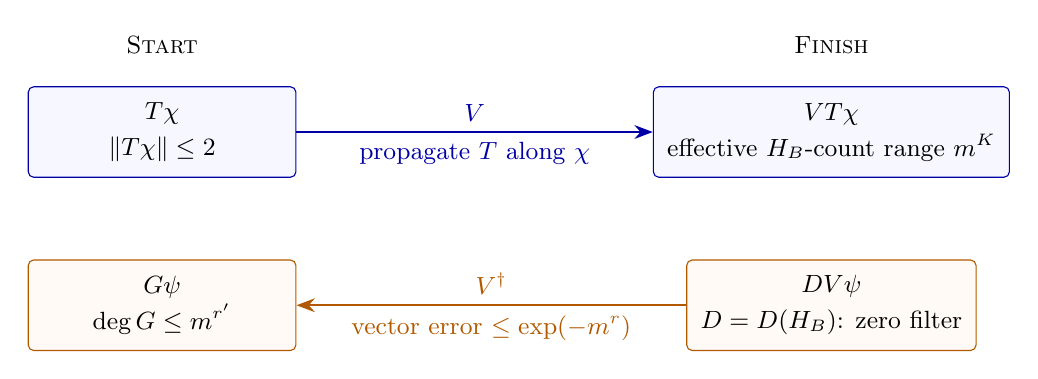
\begin{tikzpicture}[
  >=Stealth,
  every node/.style={font=\small},
  state/.style={draw,rounded corners=2pt,minimum width=3.4cm,
    minimum height=1.15cm,align=center,inner sep=5pt},
  forward/.style={state,draw=blue!65!black,fill=blue!3},
  backward/.style={state,draw=orange!70!black,fill=orange!4}
]
\node[font=\small\scshape] at (0,1.1) {Start};
\node[font=\small\scshape] at (8.5,1.1) {Finish};
\node[forward] (tstart) at (0,0)
  {$T\chi$\\[2pt] $\norm{T\chi}\le 2$};
\node[forward] (tfinish) at (8.5,0)
  {$VT\chi$\\[2pt] effective $H_B$-count range $m^K$};
\draw[->,thick,blue!65!black] (tstart) --
  node[above] {$V$}
  node[below,align=center] {propagate $T$ along $\chi$}
  (tfinish);
\node[backward] (dstart) at (0,-2.2)
  {$G\psi$\\[2pt] $\deg G\le m^{r'}$};
\node[backward] (dfinish) at (8.5,-2.2)
  {$DV\psi$\\[2pt] $D=D(H_B)$: zero filter};
\draw[->,thick,orange!70!black] (dfinish) --
  node[above] {$V^\dagger$}
  node[below,align=center] {vector error $\le\exp(-m^r)$}
  (dstart);
\end{tikzpicture}
\caption{The two transports in Lemma~\ref{lem:tail-transport}.
The forward step establishes a tail bound for $VT\chi$ outside
the count range $m^K$; the projection approximation is estimated
on this vector. The backward step acts on the unfiltered
reference $V\psi$. Its error is paired with $T\chi$, whose norm
is bounded by two.}
\label{fig:transport}
\end{figure}


The proof descends from the automatic zero tail above $m$ to the requested
threshold. At one step, a known tail bound above $m^u$ controls the tail
filter's global growth while the filter detects the new band
$m^h\le H_A\le m^u$. The following lemma supplies compatible exponent gaps
for this step.
Here $u,h$ are the exponents for the old and new count thresholds,
with tail precision exponents $u-\alpha$ and $h-\beta$.
The tail filter has suppression exponent $s$ and degree and logarithmic
norm bounds with exponent $k$, enlarged to $K$ under forward propagation;
the zero filter has precision exponent $q$ and degree and logarithmic
norm bounds with exponent $r$, enlarged to $r'$ under reverse propagation.
Finally, $v_0<v$ are initial count cutoff exponents, and $\theta$ is
the precision exponent used for the assumed input tail above $m^{v_0}$.

\begin{samepage}
\begin{lemma}[Exponent budget]
\label{lem:exponent-budget}
Suppose
\[
 0\le b<h<u\le1,
 \qquad 0<\alpha<\beta<h,
 \qquad u-h<\alpha.
\]
There are fixed exponents $q,k,K,r,r',s,v_0,v,\theta$ satisfying
\begin{gather*}
 0<h-\beta<q<r<r'<s<k<h,
 \qquad k<K<1,
 \qquad k<u-\alpha,\\
 \frac{K+q}{2}<r,
 \qquad s+\frac{u-h}{2}<k,\\
 \max\{b,r'\}<v_0<v<h,
 \qquad r'<\theta<v_0.
\end{gather*}
All these inequalities have strictly positive margins independent of
$m$.
\end{lemma}
\end{samepage}

\begin{proof}
Write $\eta=u-h$ and choose
$\alpha<\lambda<\nu<\beta$.  Set
\[
 k=u-\lambda,
 \qquad q=h-\nu.
\]
Then $q>h-\beta>0$, $k-q=\eta+\nu-\lambda>0$, and
$k<h$ because $\lambda>\alpha>\eta$.  In particular $k<1$.
Choose
\[
 0<e<\min\{\nu-\lambda,1-k\},
 \qquad K=k+e.
\]
The interval available for the remaining filter exponents has width
\[
 w=\left(k-\frac{\eta}{2}\right)-\frac{K+q}{2}
   =\frac{\nu-\lambda-e}{2}>0.
\]
With $a_0=(K+q)/2$, take
\[
 r=a_0+\frac w4,
 \qquad r'=a_0+\frac w2,
 \qquad s=a_0+\frac{3w}{4}.
\]
Thus
\[
 r-a_0=r'-r=s-r'=k-s-\frac\eta2=\frac w4>0.
\]
These choices give $q<r<r'<s<k<h$, as well as
$k<u-\alpha$.  Since $\max\{b,r'\}<h$, choose $v_0,v$
strictly between these endpoints in the stated order and then choose
$r'<\theta<v_0$.  Each choice is made among fixed real numbers.
\end{proof}

\begin{proof}[Proof of Lemma~\ref{lem:tail-transport}]
Fix target exponents $b<h_*<1$ and $0<p_*<h_*$.  Set
\[
 \delta=\frac{h_*-p_*}{4},
 \qquad
 N=\left\lceil\frac{2(1-h_*)}{\delta}\right\rceil,
 \qquad \eta=\frac{1-h_*}{N}.
\]
Here $N\ge1$ is fixed and $0<\eta\le\delta/2$.  Define
\[
 h_i=1-i\eta,
 \qquad \alpha_i=\delta+\frac{i\delta}{N}
 \qquad (0\le i\le N).
\]
We descend from $h_0=1$ to $h_N=h_*$, proving at step $i\ge1$ that
\[
 \norm{\one_{H_A\ge m^{h_i}}\chi}
 \le\exp\bigl(-m^{h_i-\alpha_i}\bigr).
\]
To start, the tail \emph{strictly above} $m^{h_0}=m$ is zero,
since the spectrum of $H_A$ is contained in $\{0,\ldots,m\}$.
No estimate on the eigenspace of count $m$, and no regularity condition
at exponent one, is needed.

Fix a step and abbreviate
\[
 u=h_{i-1},\qquad h=h_i,\qquad
 \alpha=\alpha_{i-1},\qquad \beta=\alpha_i.
\]
Its induction hypothesis is
\[
 \norm{\one_{H_A>m^u}\chi}
 \le\exp\bigl(-m^{u-\alpha}\bigr).
\]
For $i>1$ this follows from the preceding, stronger inclusive bound.
The parameters obey the hypotheses of Lemma~\ref{lem:exponent-budget}:
indeed, $u-h=\eta<\delta\le\alpha$ and
$\beta\le2\delta<h_*\le h$.  Choose its exponents once for this
step.  All subsequent estimates are for sufficiently large $m$.

\emph{Forward propagation on the trajectory of $\chi$.}
Apply Lemma~\ref{lem:tail-filter} with parameters $v,h,u,s,k$, and
write $T=T(H_A)$ for its polynomial evaluated at the initial count.
It is self-adjoint and nonnegative.  Its degree is at most $m^k$,
its global norm is at most $\exp(m^k)$, and
\[
 \norm{\one_{H_A\le m^v}T\chi}\le\exp(-m^s),
\]
because $\norm{\chi}\le1$.  Splitting at the previous scale gives
\begin{align*}
 \norm{T\chi}
 &\le \norm{\one_{H_A\le m^u}\chi}
       +\norm{T}\,\norm{\one_{H_A>m^u}\chi}\\
 &\le 1+\exp\bigl(m^k-m^{u-\alpha}\bigr)
 \le2.
\end{align*}
This is the first use of a global polynomial norm; it is paid for by
$k<u-\alpha$.

Proposition~\ref{prop:propagation}, applied with exponents $k<K$ to
the regular reference trajectory from $\chi$, gives an operator $E$
such that
\[
 \norm{VT\chi-EV\chi}\le\exp(-m^k),
 \qquad \deg E\le m^K,
 \qquad \norm{E}\le\exp(m^K).
\]
The endpoint $V\chi=P_BV\psi$ has exactly zero $H_B$ count.
By Lemma~\ref{lem:degree-shift},
$\one_{H_B>m^K}EV\chi=0$.  Therefore the filtered vector has the
effective-range bound
\[
 \norm{\one_{H_B>m^K}VT\chi}\le\exp(-m^k).
\]

\emph{Approximating the final projection on the controlled side.}
Use Lemma~\ref{lem:zero-filter} with precision exponent $q$, range
exponent $K$, and degree exponent $r$.  These satisfy $0<q<K<1$
and $r>(K+q)/2$.  Write $D=D(H_B)$ for the resulting self-adjoint
operator.  It has degree at most $m^r$, norm at most $\exp(m^r)$,
and error at most $\exp(-m^q)$ from $P_B$ on every integer count
at most $m^K$.  The preceding bound and $\norm{VT\chi}\le2$ imply
\begin{align*}
 \norm{(P_B-D)VT\chi}
 &\le 2\exp(-m^q)
       +\bigl(1+\exp(m^r)\bigr)\exp(-m^k)\\
 &=O\bigl(\exp(-m^q)\bigr).
\end{align*}
Here $q<r<k$ absorbs the global norm of $D$ on the remaining tail.
Only integer approximation is used, as required for the spectrum of
$H_B$.

Let $a_m=\ip{\chi}{T\chi}\ge0$.  Since $T$ is self-adjoint and
$V\chi=P_BV\psi$,
\[
 a_m=\ip{VT\chi}{P_BV\psi}.
\]
Moving the self-adjoint difference $P_B-D$ to the first argument
gives
\begin{align*}
 \abs{a_m-\ip{VT\chi}{DV\psi}}
 &=\abs{\ip{(P_B-D)VT\chi}{V\psi}}\\
 &\le\norm{(P_B-D)VT\chi}\,\norm{V\psi}
 =O\bigl(\exp(-m^q)\bigr).
\end{align*}
Thus the projection is approximated on $VT\chi$, the vector for which
an effective count range has just been proved.

\emph{Reverse propagation on the trajectory of $\psi$.}
The reversed trajectory starting at $V\psi$ is regular for
$V^\dagger$.  Applying Proposition~\ref{prop:propagation} to $D$
with exponents $r<r'$ gives an operator $G$ satisfying
\[
 \norm{V^\dagger DV\psi-G\psi}\le\exp(-m^r),
 \qquad \deg G\le m^{r'},
 \qquad \norm{G}\le\exp(m^{r'}).
\]
This application uses the unfiltered reference vector $V\psi$.
In the scalar product its error is multiplied by the vector norm
$\norm{T\chi}\le2$, so
\[
 \abs{a_m-\ip{T\chi}{G\psi}}
 \le O\bigl(\exp(-m^q)\bigr)+2\exp(-m^r)
 =O\bigl(\exp(-m^q)\bigr).
\]
The global operator norm of $T$ introduces no factor here.

\emph{Splitting the scalar product by the initial count.}
Put $Q=\one_{H_A\le m^v}$.  Its low-count contribution satisfies
\[
 \abs{\ip{QT\chi}{QG\psi}}
 \le\exp(-m^s)\,\exp(m^{r'}).
\]
For the high-count contribution, first observe that
$m^{v_0}+m^{r'}<m^v$ eventually.  The degree-shift property implies
\[
 (I-Q)G\one_{H_A\le m^{v_0}}=0.
\]
Using \eqref{eq:input-tail} with threshold exponent $v_0>b$
and precision exponent $\theta<v_0$ gives
\begin{align*}
 \norm{(I-Q)G\psi}
 &\le\norm{G}\,\norm{\one_{H_A>m^{v_0}}\psi}\\
 &\le\exp\bigl(m^{r'}-m^\theta\bigr).
\end{align*}
Orthogonality of $Q$ and $I-Q$ now yields
\begin{align*}
 \abs{\ip{T\chi}{G\psi}}
 &\le\exp\bigl(m^{r'}-m^s\bigr)
      +2\exp\bigl(m^{r'}-m^\theta\bigr)\\
 &=O\bigl(\exp(-m^q)\bigr),
\end{align*}
since $s>r'>q$ and $\theta>r'>q$.  These two strict gaps pay for
the two uses of the global norm of $G$.  In particular there is a
constant $C_0$, independent of $m$, with
\[
 0\le a_m\le C_0\exp(-m^q)
\]
eventually.  No commutation between $G$ and the count projections has
been assumed.

\emph{Positivity and descent.}
The tail filter is at least $1/4$ on $[m^h,m^u]$ and nonnegative
on the entire spectrum.  Consequently
\[
 \norm{\one_{m^h\le H_A\le m^u}\chi}^2
 \le4a_m\le4C_0\exp(-m^q).
\]
Combining this band with the previous upper tail gives
\[
 \norm{\one_{H_A\ge m^h}\chi}^2
 \le4C_0\exp(-m^q)
       +\exp\bigl(-2m^{u-\alpha}\bigr).
\]
Set $a=h-\beta>0$.  The exponent budget gives $q>a$, and
$u-\alpha-a=(u-h)+(\beta-\alpha)>0$.  Multiplying the last
right-hand side by $\exp(2m^a)$ therefore makes both terms tend to
zero.  Taking the square root proves
\[
 \norm{\one_{H_A\ge m^h}\chi}\le\exp(-m^{h-\beta})
\]
eventually, closing the descending step.  The strict power gap $q>a$
absorbs the square root and all fixed constants.

There are only $N$ descending steps.  Each uses
Proposition~\ref{prop:propagation} over the same bounded number of
layers with fixed positive exponent gaps $K-k$ and $r'-r$.
These gaps can be subdivided into that fixed number of positive
increments as in its proof.  Different descending steps retain only
the improved tail assertion; their approximating operators are not
composed.  Thus every choice and every number of steps is independent
of $m$, and the finitely many eventual estimates hold simultaneously
after increasing the threshold for $m$.

At the final scale,
\[
 h_N-\alpha_N=h_*-2\delta
 =\frac{h_*+p_*}{2}>p_*.
\]
The final induction bound implies the desired estimate at $h_*,p_*$.
Since these targets were arbitrary, the lemma follows.
\end{proof}

\section{Projection insertion and pruning}\label{sec:pruning}

The tail-transport lemma assumes regularity of two trajectories.  We first
use it on successively longer suffixes to show that inserting a product
projection preserves regularity.  Two consequences for product starting
states will then allow us to construct regular trajectories by deleting
reflections with small projection probability. Gate deletion by a
telescoping estimate also appears in the Pauli-spectrum approach of
\citet[Lemma~23 and Claim~24]{NadimpalliParhamVasconcelosYuen2024},
where width controls a Frobenius-norm error. Here deletion depends on
projection probability in the actual pruned-prefix state; the retained
layer must then satisfy the regularity condition for every fixed
exponent triple.

\begin{proposition}[Projection insertion]\label{prop:projection-insertion}
Let $W=U_t\cdots U_1$ have a bounded number of layers, and suppose the
trajectory
\[
 \psi_j=U_j\cdots U_1\psi_0,\qquad 0\le j\le t,
\]
is regular, with $\norm{\psi_0}\le1$.  For any product test $B$ at the
output, set
\[
 \chi_t=P_B\psi_t,\qquad
 \chi_j=U_{j+1}^{\dagger}\cdots U_t^{\dagger}\chi_t
 \quad(0\le j<t).
\]
Then the trajectory $(\chi_j)_{j=0}^t$ is regular for $W$.
\end{proposition}

\begin{proof}
All the vectors $\chi_j$ have norm at most one.  We prove their regularity
at the layers in decreasing order of the layer index.  Suppose regularity
has already been established at every layer strictly after layer $j$.
There is nothing to prove if $U_j$ is a layer of one-qubit unitaries.
Otherwise, fix $0\le b<1$ and choose, at each member of the circuit
sequence, a set $S$ of at most $m^b$ reflections in this layer.  Let
$H_A=H_S$ be their joint count and put
\[
 V=U_t\cdots U_{j+1}.
\]
This is the suffix \emph{strictly after} layer $j$, and
$\chi_j=V^{\dagger}P_BV\psi_j$.  The trajectory of $\psi_j$ on $V$ is
regular by hypothesis; that of $\chi_j$ on $V$ is regular by the
induction hypothesis.  Regularity of the original trajectory at layer
$j$ also gives, for every fixed $b<h<1$ and $0<p<h$,
\[
 \norm{\one_{H_A\ge m^h}\psi_j}\le \exp(-m^p)
 \quad\text{eventually}.
\]
Lemma~\ref{lem:tail-transport} therefore gives the same estimate for
$\chi_j$.  The count $H_S$ commutes with every reflection of layer $j$,
so this estimate holds on $\chi_{j-1}$ as well.

The chosen sets $S$ may vary with the circuit sequence.  For each fixed
triple $(b,h,p)$, Lemma~\ref{lem:uniformization} consequently makes the
estimate eventual and uniform over all eligible $S$.  This proves
regularity at layer $j$ and completes the induction.  Its first step
uses the empty suffix, whose regularity hypotheses are vacuous.
\end{proof}

\begin{corollary}[Tail at a product input]\label{cor:product-tail}
Suppose $\psi_0$ is a normalized product state and its trajectory under
$W$ is regular.  Let $P_0=|\psi_0\rangle\langle\psi_0|$ be the full
product projection and $H_0$ its count.  For any product test $B$ at the
output and every fixed $0<p<h<1$,
\begin{equation}\label{eq:product-tail}
 \norm{\one_{H_0\ge m^h}W^{\dagger}P_BW\psi_0}
 \le \exp(-m^p)
 \quad\text{eventually}.
\end{equation}
\end{corollary}

\begin{proof}
The original trajectory is regular by assumption and the projected
trajectory is regular by Proposition~\ref{prop:projection-insertion}.
Since $H_0\psi_0=0$, the input-tail hypothesis of
Lemma~\ref{lem:tail-transport} holds with $b=0$.  Applying that lemma to
$V=W$ proves the claim.
\end{proof}

\begin{corollary}[Overlap and output tail]\label{cor:overlap-tail}
Under the hypotheses of Corollary~\ref{cor:product-tail}, write
$\psi_t=W\psi_0$.  For any product test $B$ at the output and every
fixed $0<p<h<1$,
\begin{equation}\label{eq:overlap-tail}
 \norm{P_B\psi_t}^{2}
 \norm{\one_{H_B\ge m^h}\psi_t}
 \le \exp(-m^p)
 \quad\text{eventually}.
\end{equation}
For each fixed $(h,p)$, both this estimate and
\eqref{eq:product-tail} hold eventually uniformly over the output test
$B$.
\end{corollary}

\begin{proof}
Put $\chi_t=P_B\psi_t$ and $q_B=\norm{P_B\psi_t}^2$.  Apply
Lemma~\ref{lem:tail-transport} to the reverse circuit $V=W^{\dagger}$,
starting at $\chi_t$, with initial count $H_B$ and final projection
$P_0$.  The starting vector has zero $H_B$ count.  Its trajectory is
regular by Proposition~\ref{prop:projection-insertion} and reversal.
The projected-and-returned vector is exactly
\begin{align*}
 W P_0 W^{\dagger}\chi_t
 &=\psi_t\,\ip{\psi_0}{W^{\dagger}P_BW\psi_0}\\
 &=q_B\psi_t.
\end{align*}
Its reverse trajectory is the original trajectory multiplied by
$q_B\in[0,1]$, hence is regular too.  The lemma, with $b=0$, now gives
\eqref{eq:overlap-tail}.  In particular, the multiplier is the
\emph{probability} $q_B$, not its square root: no projected vector has
been normalized.

For uniformity, fix $(h,p)$ and suppose that either estimate fails for
some test at arbitrarily large indices.  Choose a violating test at
those indices and any test at the others.  The resulting single
sequence of tests contradicts the estimate just proved.  Thus tests
may be selected using the exact circuit and its output state.  The
threshold may depend on the fixed exponents; no threshold uniform over
all real exponent pairs is asserted.
\end{proof}

\newpage
\begin{lemma}[A retained layer is regular]\label{lem:retained-layer}
Let $W$ have a regular trajectory from a normalized product state, and
write $\psi=W\psi_0$.  Consider a proposed next layer of disjoint
reflections $I-2P_g$.  Retain precisely the gates satisfying
\begin{equation}\label{eq:retention-rule}
 q_g:=\norm{P_g\psi}^{2}\ge m^{-6}.
\end{equation}
The retained layer is regular on $\psi$, and hence after its action on
$\psi$ as well.
\end{lemma}

\begin{proof}
The mean bound and Markov's inequality put substantial mass on
low-weight product-basis outcomes. Counting these outcomes yields
one of sufficiently large probability; recentering the test there
changes every count by at most the outcome's weight, so
Corollary~\ref{cor:overlap-tail} supplies the required tail estimate.

We first bound the mean count of each retained gate.  Fix $\epsilon>0$
and choose fixed exponents $0<p_0<h_0<\min\{\epsilon,1\}$.  Applied to
the test of a retained gate, \eqref{eq:overlap-tail} gives
\[
 \norm{\one_{H_g\ge m^{h_0}}\psi}
 \le m^6\exp(-m^{p_0}).
\]
Since $0\le H_g\le mI$ and $\norm{\psi}=1$, spectral decomposition
therefore gives
\begin{equation}\label{eq:retained-mean}
 \ip{\psi}{H_g\psi}
 \le m^{h_0}+m^{13}\exp(-2m^{p_0})
 \le m^{\epsilon}
 \quad\text{eventually}.
\end{equation}
Corollary~\ref{cor:overlap-tail} makes this bound uniform over the
retained gates.

Now fix a regularity triple $0\le b<h<1$, $0<p<h$, and choose
$\epsilon>0$ so that $b+2\epsilon<h$.  For any set $S$ of at most
$m^b$ retained gates, disjointness of the supports gives
\[
 H_S=\sum_{g\in S}H_g,
 \qquad
 \ip{\psi}{H_S\psi}\le m^{b+\epsilon}.
\]
The empty set has zero tail, so we may suppose $S$ is nonempty.
Consider the distribution obtained by measuring the tested sites in
the product basis consisting of each specified state and its
orthogonal complement.  Label the outcomes by
binary strings, with $0$ for the specified state.  The Hamming weight
of the resulting string is the measured value of $H_S$.  With
\[
 R=2m^{b+\epsilon},\qquad \beta=b+2\epsilon,
\]
Markov's inequality puts at least half the probability on strings of
weight at most $R$.  If $M\le m$ sites are tested, the number $N_R$ of
such strings satisfies, eventually,
\begin{align*}
 N_R\le\sum_{j=0}^{\lfloor R\rfloor}\binom mj
 &\le (\lfloor R\rfloor+1)m^{\lfloor R\rfloor},\\
 \log(2N_R)&=O(m^{b+\epsilon}\log m)=o(m^{\beta}).
\end{align*}
Consequently one such outcome $z$ has probability
\begin{equation}\label{eq:pruning-atom}
 \rho\ge\frac{1}{2N_R}\ge\exp(-m^{\beta})
 \quad\text{eventually}.
\end{equation}
Only linearity of the mean, Markov's inequality, and counting have
been used; the outcomes need not be independent.

Let $B$ specify the local states of $z$ on the tested sites and leave
all other sites unconstrained.  Then $\rho=\norm{P_B\psi}^2$.
The operators $H_B$ and $H_S$ are diagonal in the same product basis.
At a site where $z$ is $0$ their count terms agree; at a site where
$z$ is $1$ they differ by an operator of norm one.  Thus their
eigenvalues on every common basis vector differ by at most
$|z|\le R$.  Choose fixed exponents
\[
 \max\{p,\beta\}<p'<h'<h.
\]
Because $b+\epsilon<h'<h$, eventually
$m^h-R\ge m^{h'}$.  The common basis then gives the spectral inclusion
\[
 \one_{H_S\ge m^h}\le\one_{H_B\ge m^{h'}}.
\]
Apply \eqref{eq:overlap-tail} to $B$ with exponents $(h',p')$, and
divide by its probability from \eqref{eq:pruning-atom}:
\begin{align*}
 \norm{\one_{H_S\ge m^h}\psi}
 &\le\norm{\one_{H_B\ge m^{h'}}\psi}\\
 &\le\rho^{-1}\exp(-m^{p'})\\
 &\le\exp(m^{\beta}-m^{p'})
 \le\exp(-m^p)
 \quad\text{eventually}.
\end{align*}
The last inequality uses both $p'>\beta$ and $p'>p$.

For each fixed target triple, the preceding bounds are uniform over
$S$ and its selected outcome $z$.  Indeed the endpoint estimate is
uniform over all product tests, including those selected from the
current state.  Equivalently, a sequence of violating choices would
contradict Corollary~\ref{cor:overlap-tail} on that subsequence.  Only
finitely many auxiliary exponent choices were made for this triple.
All uses of the corollary concern the already regular prefix $W$;
the proposed next layer is not among its hypotheses.  We have proved
regularity before the retained layer, and commutation of $H_S$ with
that layer gives the same property afterward.
\end{proof}

\begin{proposition}[Pruning from a product state]\label{prop:pruning}
For any sequence of circuits $U=U_t\cdots U_1$ on $m$ qubits, with a
bounded number $t$ of analytic layers, and any normalized product
starting states $\psi_0$, the following construction produces a
circuit $W$ with a regular trajectory from $\psi_0$.  Leave all
one-qubit layers unchanged.  At a reflection layer, use the exact
state reached by the pruned prefix and retain exactly the gates in
\eqref{eq:retention-rule}.  The output vectors satisfy
\begin{equation}\label{eq:pruning-error}
 \norm{U\psi_0-W\psi_0}\le 2t m^{-2}.
\end{equation}
\end{proposition}

\begin{proof}
The empty prefix is regular.  Appending a one-qubit layer adds no
regularity condition, and Lemma~\ref{lem:retained-layer} applies at
each reflection layer.  Induction therefore gives regularity of the
whole pruned trajectory.  The retention rule itself has no exponent
choices: the auxiliary exponents above are used only to verify its
regularity for each fixed triple.

For the error estimate, denote the retained version of layer $U_j$ by
$\widetilde U_j$ and the exact pruned-prefix state before it by
$\psi_{j-1}$.  Each deleted reflection $F_g=I-2P_g$ satisfies
\[
 \norm{(F_g-I)\psi_{j-1}}
 =2\norm{P_g\psi_{j-1}}<2m^{-3}.
\]
Every other gate in that layer commutes with $P_g$, and is unitary.
Hence this norm is unchanged if any other gates of the layer have
already acted.  Telescoping over the deleted gates, of which there
are at most $m$ because their nonempty supports are disjoint, yields
\[
 \norm{(U_j-\widetilde U_j)\psi_{j-1}}\le2m^{-2}.
\]
This bound is zero for a one-qubit layer.  If $\phi_j$ and $\psi_j$
are the original and pruned states after layer $j$, respectively,
then exactly
\[
 \phi_j-\psi_j
 =U_j(\phi_{j-1}-\psi_{j-1})
   +(U_j-\widetilde U_j)\psi_{j-1}.
\]
Unitarity and the triangle inequality give
$\norm{\phi_j-\psi_j}\le\norm{\phi_{j-1}-\psi_{j-1}}+2m^{-2}$.
Starting with $\phi_0=\psi_0$ proves \eqref{eq:pruning-error}.
\end{proof}

\section{The parity contradiction}\label{sec:parity}

We now prove Theorem~\ref{thm:parity}.  Reference qubits retain the
classical input labels while the computation may freely change all
its own registers.  Their signed acceptance expectation will be
bounded away from zero by correctness and forced to zero by
Corollary~\ref{cor:product-tail}.

\begin{proof}[Proof of Theorem~\ref{thm:parity}]
Fix positive integers $d,k,C$ and $0<\varepsilon\le1/2$, where $k$ is
now the resource exponent in the theorem. Suppose, toward a contradiction, that an unbounded
set of input lengths $n$ admits a depth-at-most-$d$ circuit $U$ with
at most $C(n+1)^k$ total qubits,
whose success probability is at least $1/2+\varepsilon$ on every input. Choose
one such circuit at each member of an increasing sequence of lengths.
Write $a$ for its number of ancillary qubits and $I$ for its $n$
input qubits.

Attach a register $R$ of $n$ reference qubits, initially zero, and
let $\operatorname{COPY}$ be the layer of disjoint CNOTs from input
qubit $I_i$ to reference qubit $R_i$.  Our normalized product starting
state is
\[
 \psi_0=|+\rangle_I^{\otimes n}
          \otimes|0\rangle^{\otimes a}
          \otimes|0\rangle_R^{\otimes n},
 \qquad |+\rangle=\frac{|0\rangle+|1\rangle}{\sqrt2}.
\]
The enlarged circuit $(U\otimes I_R)\operatorname{COPY}$ has
$m=2n+a$ qubits.  Splitting the original layers into the two analytic
types of Section~\ref{sec:framework} gives at most $t=2d+1$ layers,
including the copying layer.  In particular the layer count is
bounded, $m\to\infty$, and, since $k\ge1$,
\begin{equation}\label{eq:parity-resources}
 m=2n+a\le(C+2)(n+1)^k.
\end{equation}

Apply Proposition~\ref{prop:pruning} to this circuit and $\psi_0$,
and call the pruned circuit $W$.  Every copying gate is retained for
all sufficiently large $m$.  Indeed its reflection projection is
\[
 P_g=|1\rangle\langle1|_{I_i}
       \otimes|-\rangle\langle-|_{R_i},
 \qquad |-\rangle=\frac{|0\rangle-|1\rangle}{\sqrt2},
\]
and its probability on $\psi_0$ is
$|\langle1|+\rangle|^2|\langle-|0\rangle|^2=1/4\ge m^{-6}$
eventually.  All later gates avoid $R$, so we can write
\[
 W=(\widetilde U\otimes I_R)\operatorname{COPY}
\]
for a circuit $\widetilde U$ on the original qubits.  Let
\[
 \Phi=(U\otimes I_R)\operatorname{COPY}\psi_0,
 \qquad \Omega=W\psi_0.
\]
Both states are normalized, the trajectory to $\Omega$ is regular,
and \eqref{eq:pruning-error} gives
$\norm{\Phi-\Omega}\le2t m^{-2}$.

Let $P_B$ project the designated answer qubit onto $|1\rangle$, and
let $Z_R=\prod_{i=1}^n Z_{R_i}$.  The answer qubit belongs to the
original circuit and may be one of its input qubits; in either case
$P_B$ acts outside $R$ and commutes with $Z_R$.  Set
$p_x=\Pr_U(1\mid x)$.  The original coherent output is
\[
 \Phi=2^{-n/2}\sum_{x\in\{0,1\}^n}
        U\bigl(|x\rangle_I\otimes|0\rangle^{\otimes a}\bigr)
        \otimes|x\rangle_R.
\]
The reference states are orthogonal, so
\begin{equation}\label{eq:parity-correlation}
 \ip{\Phi}{Z_RP_B\Phi}
 =2^{-n}\sum_x(-1)^{|x|}p_x
 \le\frac12\!\left(\left(\frac12-\varepsilon\right)
                  -\left(\frac12+\varepsilon\right)\right)
 =-\varepsilon.
\end{equation}
Here $p_x\le1/2-\varepsilon$ on even-parity inputs and
$p_x\ge1/2+\varepsilon$ on
odd-parity inputs, and there are equally many of each for $n\ge1$.

The self-adjoint observable $Z_RP_B$ has norm at most one.  For any
two unit vectors its expectation changes by at most twice their
distance, by expanding the difference in its two arguments.  Hence
\begin{equation}\label{eq:pruned-correlation}
 \ip{\Omega}{Z_RP_B\Omega}
 \le-\varepsilon+4t m^{-2}.
\end{equation}
Thus approximating this one coherent state transfers the signed
expectation needed below.  No success claim for $\widetilde U$ on
individual basis inputs is required.

Because $\widetilde U$ acts trivially on $R$, and a CNOT conjugates
$Z$ on its target to the product of $Z$ on control and target,
\begin{equation}\label{eq:reference-conjugation}
 W^{\dagger}Z_RW
 =\operatorname{COPY}^{\dagger}Z_R\operatorname{COPY}
 =Z_I Z_R,
 \qquad Z_I=\prod_{i=1}^n Z_{I_i}.
\end{equation}
The one-pair conjugation identity follows directly on a basis vector:
the target bit after copying is $r_i\mathbin{\oplus}x_i$, so its
$Z$ eigenvalue is $(-1)^{r_i+x_i}$.  Acting on $\psi_0$, the last
operator in \eqref{eq:reference-conjugation} gives
\[
 \psi'_0=W^{\dagger}Z_RW\psi_0
 =|-\rangle_I^{\otimes n}
       \otimes|0\rangle^{\otimes a}
       \otimes|0\rangle_R^{\otimes n}.
\]
Let $H_0$ be the count associated with the full product state
$\psi_0$.  Every input factor of $\psi'_0$ is orthogonal to its
specified $|+\rangle$ state, while all other factors agree with their
specified states.  Consequently
\[
 \norm{\psi'_0}=1,\qquad H_0\psi'_0=n\psi'_0.
\]
Moving the unitary and $Z_R$ across the inner product gives
\begin{equation}\label{eq:parity-pairing}
 \ip{\Omega}{Z_RP_B\Omega}
 =\ip{\psi'_0}{W^{\dagger}P_BW\psi_0}.
\end{equation}
This identity does not require commuting $P_B$ through $W$ or
preserving an input register.

Choose fixed exponents
\[
 0<p<h<\min\{1,1/k\}.
\]
By \eqref{eq:parity-resources}, $m^h=O(n^{kh})=o(n)$, so
$m^h<n$ eventually.  The vector $\psi'_0$ then belongs to the range
of $\one_{H_0\ge m^h}$.  Cauchy--Schwarz and
Corollary~\ref{cor:product-tail}, applied to the regular trajectory
of $W$, show that
\[
 \left|\ip{\Omega}{Z_RP_B\Omega}\right|
 \le\norm{\one_{H_0\ge m^h}W^{\dagger}P_BW\psi_0}
 \le\exp(-m^p).
\]
This tends to zero, contradicting \eqref{eq:pruned-correlation}.

For the fixed $d,k,C,\varepsilon$, let $\mathcal S$ be the set of input lengths
admitting an admissible circuit with success at least $1/2+\varepsilon$ on every
input.  The contradiction excludes an unbounded $\mathcal S$;
hence $\mathcal S$ is finite.  There is therefore a threshold
$n_0=n_0(d,k,C,\varepsilon)$ such that at every $n\ge n_0$, every circuit meeting
the specified depth and total-qubit bounds has an input on which
its success probability is strictly less than $1/2+\varepsilon$. In particular,
for every positive integer $N$, every $n\ge\max\{N,n_0\}$ has
this failure property.  This proves
Theorem~\ref{thm:parity} with the stated strict failure threshold.
\end{proof}

\paragraph{Majority and symmetric-function consequences.}
Xu and Li's Theorem~1 and Corollaries~2--3
\citep{XuLi2026Fanout}, combined with Theorem~\ref{thm:parity}, also
exclude strict majority and broader symmetric families in our circuit
model. More precisely, let \(f_n:\{0,1\}^n\to\{0,1\}\) be symmetric, let \(f_{n,i}\) be its
value at Hamming weight \(i\), and set
\(\rho(f_n)=\max_{0\le i<n:\,f_{n,i}\ne f_{n,i+1}}\min\{i+1,n-i\}\), with zero
for constant functions. Its pointwise-error-\(1/3\) approximate degree is
the least total degree of a real polynomial \(p\) satisfying
\(\lvert p(x)-f_n(x)\rvert\le1/3\) for every \(x\in\{0,1\}^n\).
Assume either \(\rho(f_n)\ge n^\delta\) for all sufficiently large \(n\)
for some fixed \(\delta>0\), or this approximate degree is
\(\Omega(n^{1/2+\eta})\) for some fixed \(\eta>0\). Then no
fixed-depth, polynomial-total-qubit family achieves success at least
\(1/2+1/(\log n)^\gamma\) on every input at every sufficiently large
length, for any fixed \(\gamma>0\). Strict majority
\(\operatorname{MAJ}_n(x)=\mathbf1_{\{|x|>n/2\}}\) has
\(\rho=\lceil n/2\rceil\).

The full formulation and output-model adjustment are recorded in the
companion article
\citep[Section~7.3, Corollary~10 and its proof]{OpenAILocalization2026}.
Xu and Li require the measured output to be an initially zero ancilla.
Appending one fresh zero qubit and a CNOT from our designated output
preserves its measurement distribution even with arbitrary garbage, at a
cost of one qubit and one layer.
A family with the stated success would, after this adjustment, yield exact
clean fanout through the cited reduction. The Hadamard-to-parity argument in
Section~\ref{sec:introduction} excludes such fanout using our own
Theorem~\ref{thm:parity}. Under the same circuit conventions, adjoining
unit-cost primitive reversible unbounded threshold gates therefore
strictly enlarges the class computed with worst-case success at least
\(2/3\): the reversible gate
\(\lvert x,b\rangle\mapsto\lvert x,b\mathbin\oplus\operatorname{MAJ}_n(x)\rangle\)
computes majority exactly from a zero target.

\paragraph{State-preparation consequences.}
We justify the bounds stated in Section~\ref{sec:introduction}.
Keep every register of a preparation when using its unitary and inverse.
For felinity $\eta>0$ on $h$ retained qubits of a depth-$d$ preparation
on $M$ total qubits, the constructions in the proofs of
\citet[Lemmas~4.9 and~4.1]{GGJ2026Fourier} give target probabilities
$a\ge1/2$ on $0^h$ and $b\ge\eta^2/2$ on $1^h$, in depth $O(d+1)$
on $O(M+h)$ qubits. The square occurs because the top Fourier
coefficient has magnitude at least $\eta$, so its weight is at least $\eta^2$.

The exact step is the one-round case of
\citet[Theorem~7]{GrierMorrisWu2026}. For unit vectors $g,e$, if a
unitary $V$ prepares
$V|0\rangle=(|g,0\rangle+\sqrt3|e,1\rangle)/2$, where $|0\rangle$
denotes its entire zero input and the last qubit is a flag, then
\[
 V(I-2|0\rangle\langle0|)V^\dagger Z_{\rm flag}V|0\rangle
 =|g,0\rangle.
\]
Indeed, $\langle0|V^\dagger Z_{\rm flag}V|0\rangle=-1/2$.
A flag initialized to one can be given coefficient
$c=1/(2\sqrt{a+b})\le1$ on zero separately under the two extreme
target tests: use a one-qubit reflection sending $|1\rangle$ to
$c|0\rangle+\sqrt{1-c^2}|1\rangle$. Each conditional operation is a
product reflection, so the two tests use two sequential Toffoli gates
up to local conjugations. The flag-zero component is one half of the
normalized union of the extreme branches. The displayed identity
prepares that union exactly, with one-branch probability
$q=b/(a+b)\in[\eta^2/2,1/2]$, since $a+b\le1$ and $b\le1-a\le a$.

Prepare $r=\lceil(\log 2)/(-\log(1-q))\rceil=O(\eta^{-2})$
independent copies on fresh zeros. Disjoint columnwise reversible ORs
into $h$ new targets give probabilities
$u=(1-q)^r\in[1/4,1/2]$ on $0^h$ and $v=1-u\in[1/2,3/4]$ on $1^h$.
Here $(1-q)/2\le(1-q)^r\le1/2$ and $r\le(\log 2)/q+1$.
Giving these two branches flag-zero coefficients
$1/(2\sqrt{2u})$ and $1/(2\sqrt{2v})$, respectively, and applying
the same exact round yields
\[
 2^{-1/2}\bigl(|0^h,\alpha_0\rangle+|1^h,\alpha_1\rangle\bigr),
\]
with unit branch states $\alpha_0,\alpha_1$ containing arbitrary
garbage. The all-zero reflection is likewise a local conjugate of a Toffoli,
and the ORs use Toffoli gates with local $X$ gates. The source-dependent
flag coefficients are permitted by nonuniformity. Rosenthal's exact
case \citep[Theorem~3.1]{Rosenthal2021} converts this balanced state,
using its complete preparation and inverse, to the exact parity unitary
on arbitrary states of the $h+1$ data qubits, with every auxiliary
qubit restored to zero, and hence to clean $F_h$ by Hadamard conjugation. All copies
run in parallel, and only a constant number of preparation and
reflection stages are sequential. The resulting depth is $O(d+1)$
and the total-qubit bound is $O((M+h)\eta^{-2}+h)$.

For the Dicke bound, use the block calculation in the proof of the
companion's state-preparation corollary
\citep[Section~7.1, Corollary~8 and its proof]{OpenAILocalization2026}.
Uniformly for $n\ge2k$ and all sufficiently large $k$, it shows that
an input at trace distance at most $1/(80k)$ from $|D_k^n\rangle$
produces, with $\ell=\lfloor k/\log k\rfloor$ fresh targets and three
additional allowed layers, a retained state of felinity greater than
$1/(40k)$. Applying the preceding promotion at arity $\ell$ gives
exact parity in fixed depth on $O((M+n)k^2)$ total qubits. For fixed
$0<\delta<1$ and $k\ge n^\delta$, eventually $\ell\ge\sqrt k$, so
$n\le k^{1/\delta}\le\ell^{2/\delta}$ and $k^2\le\ell^4$ make this one fixed polynomial
bound in $\ell$. A felinity violation $\eta\ge n^{-A}$ similarly
preserves one fixed polynomial bound at arity $n$. Both parity arities
grow along any unbounded sequence of violations, contradicting the
eventual pointwise Theorem~\ref{thm:parity}.

\renewcommand{\bibsection}{%
  \section*{\refname}%
  \addcontentsline{toc}{section}{\refname}}
\setlength{\bibsep}{3pt plus .2pt minus .2pt}
\bibliographystyle{plainnat}
\bibliography{references}
\end{document}
